\chapter{Messprinzip mit Skizze und Versuchsablauf}

   	\begin{center}
    
		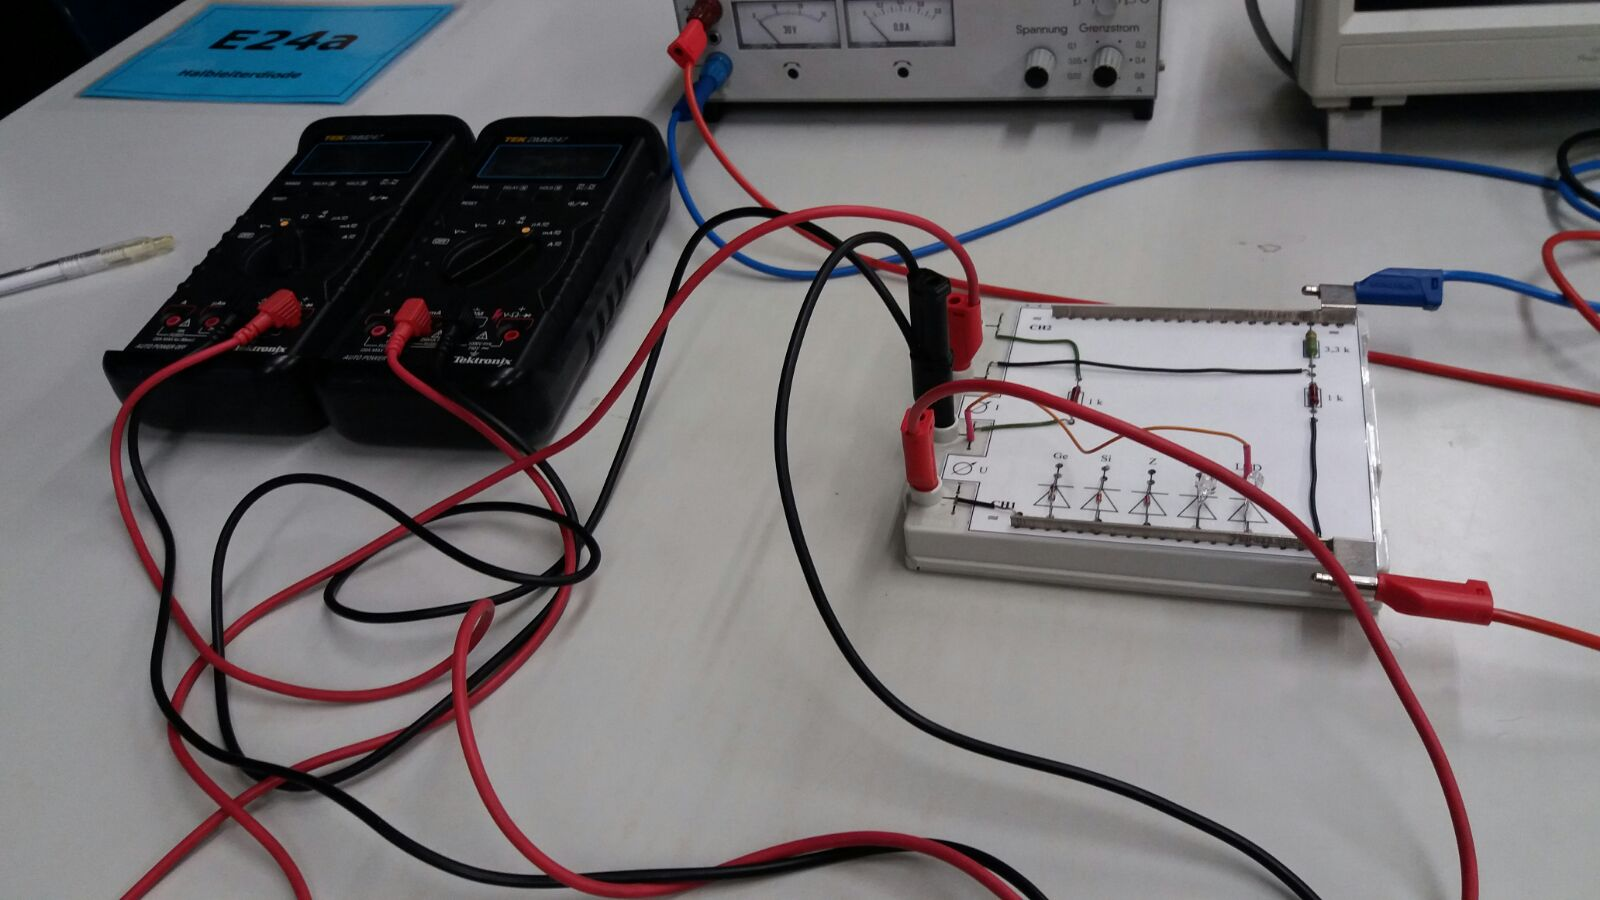
\includegraphics[scale=0.25]{Daten/Aufbau.jpg}
		\captionof{figure}[]{Versuchsaufbau}
    \end{center}
     
        
	\section{Aufgabenteil 1 a}
Im ersten Versuchsteil geht es um die Bestimmung der Kennlinien in Durchflussrichtung einer Germaniumdiode und einer Siliziumdiode. Dazu werden die Spannungen in Abhängigkeit von Strömen der Diode gemessen. Zur Bestimmung wird Gleichstrom verwendet. 
 
         \section{Aufgabenteil 1 c}
         Nachdem die Kennlinen der Germaniumdiode und der Siliziumdiode in Durchlassrichtung bestimmt wurden, wird nun die Sperrkennlinie bestimmt. Dazu werden erneut zu verschiedenen Spannungen die Ströme notiert. Dies wird erneut für beide Dioden gemacht.
         
   \section{Aufgabenteil 2}

In der zweiten Aufgabe wird erneut die Sperrkennlinie und die Durchlasskennline einer Zenerdiode bestimmt werden. Hierbei werden wie in der vorherigen Aufgabe, die Ströme und zugehörigen Spannungen bestimmt.

\section{Aufgabenteil 3}

In der letzten Aufgabe werden die Kennlinien von  zwei Leuchtdioden (rot und blau) bestimmt. Die LED wird bei Wechselstrom betrieben. Hierbei wird ein Oszilloskop zur Hilfe genommen. Die Frequenz wird dazu auf 200 Hz eingestellt. Als Format wird xy ausgewählt. Zudem muss ausgewählt werden, dass Channel 2 invertiert wird.

\pagebreak